%% Kiii Kiii — ICAIF'26 Workshop on Financial AI Security, Privacy, and Safety
%% Submission: \documentclass[sigconf,anonymous,review]{acmart}   (4 pages excl. references/appendix, double-blind)
%% Camera-ready: \documentclass[sigconf]{acmart} and remove \anonv
\documentclass[sigconf,anonymous,review]{acmart}

\usepackage{booktabs}
\usepackage{xcolor}
\usepackage{kotex}          % Korean examples in text; comment out if Overleaf compiler lacks kotex (use xelatex/lualatex)
\usepackage{enumitem}
\setlist{nosep,leftmargin=*}

%% --- anonymisation helpers: \anonv{visible}{hidden} shows the first arg in review mode
\newif\ifanonymous\anonymoustrue
\newcommand{\anonv}[2]{\ifanonymous#1\else#2\fi}   % acmart already defines \anon; ours is \anonv{visible-in-review}{camera-ready}
\newcommand{\todo}[1]{\textcolor{red}{[TODO: #1]}}

%% ACM metadata (workshop is non-archival; keep minimal)
\setcopyright{none}
\copyrightyear{2026}
\acmYear{2026}
\acmDOI{}
\acmISBN{}
\acmConference[ICAIF '26 Workshop]{Workshop on Financial AI Security, Privacy, and Safety at ICAIF '26}{November 14--15, 2026}{Milan, Italy}
\settopmatter{printacmref=false}
\renewcommand\footnotetextcopyrightpermission[1]{}

\begin{document}

\title{Kiii Kiii: A Regulation-Grounded Benchmark for Korean Financial PII Detection under Realistic Surface-Form Variation}
%% working alternatives:
%% "Beyond the Regex: Benchmarking Korean Financial PII Detection for AI Data Loss Prevention"

\author{\anonv{Anonymous Authors}{Hanwool Albert Lee}}
\affiliation{\institution{\anonv{Anonymous Institution}{AIM Intelligence}}\city{Seoul}\country{Republic of Korea}}
\email{\anonv{anonymous@example.com}{hanwool@aim-intelligence.com}}

\author{\anonv{}{Sunghyun Kim}}
\affiliation{\institution{\anonv{}{Toss Securities}}\city{\anonv{}{Seoul}}\country{\anonv{}{Republic of Korea}}}

\renewcommand{\shortauthors}{\anonv{Anonymous}{Lee and Kim}}

\begin{abstract}
AI data-loss-prevention (DLP) systems in Korean financial institutions must detect personal information whose categories are fixed by statute but whose surface forms in real text---call-centre transcripts, scanned forms, pasted tables---are anything but fixed. We introduce \textbf{Kiii-Kiii} (\emph{Korean Identifiers, Identifiability, and Ill-formed inputs}; dataset \kiii{}), a benchmark for Korean financial PII span extraction and de-identification whose name states its three axes. Its taxonomy has two tiers: a \emph{Legal} tier of 24 categories, each cited to an article of the Personal Information Protection Act, the Credit Information Act and its Enforcement Decree, the Real Name Financial Transactions Act, or the Electronic Financial Transactions Act, and an \emph{Identifiability} tier of 12 quasi-identifiers and behavioural attributes that enable profiling and hyper-personalised phishing. Documents are synthetic, long-context and multi-subject, and every identifier is generated by code with a valid checksum, then rendered through a controlled \emph{surface-form variation} axis (T0 canonical to T3 structural: dictated Korean numerals, cross-turn splitting, partial masking, agent read-back) calibrated to how commercial Korean speech-to-text engines actually emit numbers. We evaluate \todo{N} systems---regex/rule baselines, frontier APIs, open-weight models, and Korean-developed open LLMs---and find that \todo{headline finding: rules collapse at T2; Korean-native models help on X but not Y; partial-mask leakage}. The benchmark, taxonomy and generator are released \anonv{upon acceptance}{at \url{https://github.com/h-albert-lee/kiii-kiii-workspace}}.

\end{abstract}

\begin{CCSXML}
<ccs2012>
<concept><concept_id>10002978.10003029</concept_id><concept_desc>Security and privacy~Human and societal aspects of security and privacy</concept_desc><concept_significance>500</concept_significance></concept>
<concept><concept_id>10010147.10010178.10010179</concept_id><concept_desc>Computing methodologies~Natural language processing</concept_desc><concept_significance>300</concept_significance></concept>
</ccs2012>
\end{CCSXML}
\ccsdesc[500]{Security and privacy~Human and societal aspects of security and privacy}
\ccsdesc[300]{Computing methodologies~Natural language processing}
\keywords{PII detection, de-identification, data loss prevention, Korean, financial regulation, benchmark, large language models}

\maketitle

\section{Introduction}
\label{sec:intro}

\begin{figure*}[t]
  \centering
  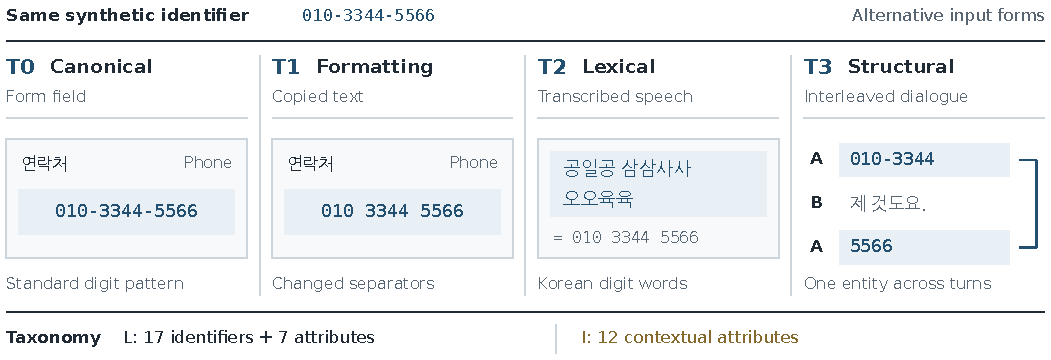
\includegraphics[width=\textwidth]{figures/fig1_overview.pdf}
  \caption{\textbf{One identifier, four input forms in \kiii{}.}
  A synthetic phone number appears in canonical (T0), formatting (T1), lexical
  (T2), and structural (T3) forms. Shading marks identifier spans; the bracket
  links speaker A's fragments across B's interruption (``mine too'').
  Examples are illustrative, not paired corpus records. The footer summarizes
  the Legal (L) and Identifiability (I) tiers.}
  \Description{Four aligned panels show the synthetic phone number
  010-3344-5566 with hyphens, with spaces, as Korean digit words, and split into
  010-3344 and 5566 across two turns by speaker A, interrupted by speaker B.
  A bracket links the two fragments. The footer summarizes 17 Legal identifiers,
  7 Legal attributes, and 12 Identifiability attributes.}
  \label{fig:overview}
\end{figure*}


%% Paragraph 1: the DLP problem. Regex solves canonical PII; real text is not canonical.
Korean financial institutions are required to prevent personal (credit) information from leaving controlled systems, and increasingly deploy LLM-based DLP filters on unstructured text. For canonical strings---a resident registration number written \texttt{900101-1234567}, a card number with a valid Luhn digit---a regular expression with a checksum is near-perfect. The difficulty is everywhere else: a customer dictating an account number as \emph{일일공 에 일이삼 에 사오육칠팔구} over the phone, a number split across two turns and read back by the agent, a scanned statement whose zeros became the letter O, a ``masked'' RRN that still exposes birth date and sex. \todo{one sentence with a concrete leakage anecdote or statistic if available}

%% Paragraph 2: why existing benchmarks do not measure this.
Existing PII benchmarks do not measure this. English benchmarks~\cite{shen2025piibench,vats2026redact} lack Korean; the only Korean PII resources are conversational~\cite{fei2024kdpii,jang2024koreanpiiner} or legal~\cite{hahm2025thunderdeid}, define categories without statutory grounding, and present identifiers in canonical form. None models how Korean speech-to-text output renders numbers, although call-centre transcripts are the largest unstructured PII stream in the sector.

%% Paragraph 3: contributions (4 bullets max).
Figure~\ref{fig:overview} illustrates the controlled input variations and taxonomy
underlying \kiii{}. We make three contributions.
\begin{enumerate}
  \item A \textbf{regulation-grounded, two-tier taxonomy} of 36 categories: 24 \emph{Legal} categories each cited to a statutory article (\S\ref{sec:taxonomy}), and 12 \emph{Identifiability} categories capturing quasi-identifiers and behavioural attributes that enable profiling.
  \item A \textbf{synthetic long-context, multi-subject corpus} in which identifiers are generated by code (checksum-valid) and rendered through a controlled \textbf{surface-form variation} axis (T0--T3) calibrated to Korean STT behaviour (\S\ref{sec:benchmark}).
  \item A \textbf{leaderboard} of \todo{N} systems spanning rule baselines, frontier APIs, open-weight and Korean-developed LLMs, with analysis by tier, variation level, subject count and context length (\S\ref{sec:results}).
\end{enumerate}

\section{Related Work}
\label{sec:related}

\paragraph{PII detection benchmarks.}
PII-Bench~\cite{shen2025piibench} evaluates query-aware masking over 55 English PII types and is the only prior work with an explicit multi-subject split, on which LLMs degrade. REDACT~\cite{vats2026redact} stratifies 25 languages by sensitivity tier and disclosure form; Mind the Gap~\cite{zafar2026mindthegap} stress-tests English detectors under seven distribution shifts. Off-the-shelf filters degrade sharply on non-Latin scripts~\cite{uppala2026opf}. Our benchmark instead combines Korean financial categories with explicit input transformations and a jurisdiction-specific annotation policy.

\paragraph{De-identification.}
The Text Anonymization Benchmark~\cite{pilan2022tab} introduced direct/quasi-identifier distinctions and risk-weighted recall, motivating separate analysis of legal identifiers and contextual attributes. LLM-based anonymisers~\cite{staab2025anonymizers,yang2025rupta} and re-identification benchmarks~\cite{krco2026ratbench} evaluate privacy--utility trade-offs in English; Pasch and Cha~\cite{pasch2025privacyutility} study pseudonymisation with back-mapping, a distinct task from the all-mentions extraction recall measured here. The closest financial de-identification work~\cite{albanese2026anonymous} is English and industry-authored.

\paragraph{Korean financial language evaluation.}
TWICE~\cite{hwang2025twice} introduces KorFinMTEB and shows that translated English benchmarks can miss Korean financial semantics. NMIXX~\cite{lee2025nmixx} studies domain-adapted Korean--English embeddings and introduces KorFinSTS for financial semantic similarity. KFinEval-Pilot~\cite{hwang2025kfineval} evaluates Korean financial knowledge, legal reasoning and toxicity; KRX Bench~\cite{son2024krx} constructs company-knowledge questions covering Korean and other markets. These studies motivate domain- and language-specific evaluation. \kiii{} complements their semantic and knowledge tasks with typed PII spans, statutory category mappings and controlled input variation.

\paragraph{Korean PII.}
KDPII~\cite{fei2024kdpii} and Jang et al.~\cite{jang2024koreanpiiner} annotate synthetic Korean dialogues with a flat 33-tag scheme and report that models recognise universal PII (email, phone) far better than Korean-specific formats. Thunder-DeID~\cite{hahm2025thunderdeid} builds a 729-label taxonomy from 6{,}700 court judgments; its financial identifiers (accounts, cards, bills) are leaves of a generic ``unique number'' bucket without format modelling, and monetary, transaction and credit attributes are absent because judgments do not contain them. Our taxonomy inverts that emphasis and excludes public institution and product names.

\paragraph{Contextual privacy and misuse.}
Contextual-integrity benchmarks~\cite{mireshghallah2024confaide,shao2024privacylens,fan2024goldcoin,li2025privacibench} ground privacy judgments in norms or in HIPAA/GDPR; attribute-inference attacks~\cite{staab2024beyond} and automated spear-phishing studies~\cite{heiding2024spearphishing} motivate our Identifiability tier but evaluate neither Korean nor finance.

\section{Taxonomy}
\label{sec:taxonomy}

%% ~0.6 page. Table 1 = compact category table. Full statute quotes → appendix / repo.
Our taxonomy has two tiers and two kinds. \textbf{Tier L (Legal)} contains only categories \emph{enumerated} by Korean statute: the Personal Information Protection Act (PIPA) \S23--24 and Enforcement Decree \S18--19 (sensitive and unique identifying information); the Credit Information Act (CIA) \S2 and its Enforcement Decree \S2, which lists 성명·주소·전화번호, e-mail and SNS addresses, the four national identification numbers, \emph{CI/DI and any identifier a credit-information company assigns to a customer} (\S2\,③), and business/corporate registration numbers (\S2\,④); the Real Name Financial Transactions Act \S4 (transaction information); and the Electronic Financial Transactions Act \S2(10) (access media) and Decree \S7\,④ (account and policy numbers, transaction records). \textbf{Tier I (Identifiability)} contains categories no statute enumerates but which act as quasi-identifiers~\cite{pilan2022tab} or, when aggregated, enable profiling and personalised social engineering; membership in Tier I is an empirical judgment, not a legal claim.

Each category is an \textbf{identifier} (a span that alone points at a person or account) or an \textbf{attribute}. CIA \S2(1)(a) defines identifying information as credit information \emph{only when combined with} transaction, creditworthiness or capacity information; we encode this as a span policy: L-identifiers and sensitive information are \nolinkurl{must_mask}, L-attributes are \nolinkurl{mask_if_linked}, and Tier I is \nolinkurl{detect_only}. Table~\ref{tab:taxonomy} lists the 36 categories (17 L-identifier, 7 L-attribute, 12 I-attribute). Staff names are annotated as PII with a \nolinkurl{subject_role} of \emph{staff}; institution and product names, biometric templates and unattributed amounts are excluded.

\begin{table}[t]
\caption{Taxonomy overview: all 36 categories, with abbreviated labels. L denotes Legal and I denotes Identifiability.}
\label{tab:taxonomy}
\small
\begin{tabularx}{\columnwidth}{@{}>{\RaggedRight\arraybackslash}p{0.23\columnwidth}>{\RaggedRight\arraybackslash}X@{}}
\toprule
\textbf{Tier / kind} & \textbf{Categories} \\
\midrule
L / identifier\newline (17) & name; RRN; foreigner reg.\ no.; passport; driver's licence; phone; address; e-mail; online handle; customer ID; business reg.\ no.; corporate reg.\ no.; bank account; securities account; card; contract no.; access credential. \\
\addlinespace
L / attribute\newline (7) & credit transaction; transaction record; delinquency; financial capacity; credit score; public record; sensitive information. \\
\addlinespace
I / attribute\newline (12) & DOB/age; gender; nationality; family relation; employer/position; education; life event; investment profile; consultation content; service usage; device/IP; location mention. \\
\bottomrule
\end{tabularx}
\par\smallskip
\begin{minipage}{\columnwidth}
\RaggedRight\small
\textit{Policies.} L identifiers and sensitive information: must mask.
Other L attributes: mask if linked. I attributes: detect only.
Full subtypes, statutory citations and format rules are in the taxonomy specification.
\end{minipage}
\end{table}

\section{Benchmark Construction}
\label{sec:benchmark}

\paragraph{Slot-filling generation.}
Gold spans must be exact for a benchmark to be meaningful; LLM-annotated PII corpora are not (88\% of card numbers in KDPII fail Luhn validation). We therefore never let the LLM write an identifier. An LLM composes each document from a plan (document type, number of subjects, target length, variation level) using typed slots such as \texttt{\{\{bank\_account\_no:1:bank=신한\}\}} for identifiers and inline tags \texttt{[[credit\_transaction:1]]…[[/…]]} for attribute spans. Code then fills every slot with a checksum-valid value (RRN, business and corporate registration numbers, Luhn card numbers; bank-specific account templates), records character offsets and entity identity, and rejects any document in which an unslotted identifier pattern appears. Ten financial document types are covered (KYC forms, statements, loan contracts, insurance claims, call-centre transcripts, complaint records, securities reports, internal memos, phishing reports).

\paragraph{Surface-form variation (Figure~\ref{fig:overview}).}
Each document is assigned a level: \textbf{T0} canonical (regex-catchable), \textbf{T1} formatting (separator changes, regrouping, partial masking, affixes), \textbf{T2} lexical (Korean-numeral dictation \emph{공일공 삼삼사사}, Hanja/fullwidth digits, OCR confusables, STT digit errors, leftover spoken separators \emph{에}/\emph{다시}), and \textbf{T3} structural (a value split across turns, agent read-back, missing or wrong keyword anchors, coreference-only mentions, multi-subject interleaving, tables, negated/hypothetical mentions). Every gold span records its applied operations and whether it remains regex-catchable. Levels T2--T3 for transcripts follow a profile derived from commercial Korean STT behaviour: ReturnZero applies inverse text normalisation by default and CLOVA and Google emit Arabic digits with no switch, so 70\% of transcript numbers are digits; KsponSpeech and AI~Hub customer-service corpora retain a phonetic Hangul layer, so 20\% are dictated; Whisper fragments numbers, so 10\% are inconsistent. Because no commercial engine masks Korean PII at transcription time, a 20\% subset reproduces regex-masked transcripts in which dictated and split numbers survive. Intentional encoding (base64, homoglyphs) is out of scope as an attack distribution. Hard negatives (look-alike order numbers, checksum-invalid values, public hotline numbers, dates shaped like RRN prefixes, placeholders, unattributed amounts) are injected at 30\% of gold-span count.

\paragraph{Corpus.}
\todo{N docs; stratified 10 types × 4 levels × subjects \{1,3,8\} × length \{1k,4k,16k\}; 80\% composed by \anonv{a frontier API model}{gpt-5.6-sol}, 20\% by a local model to measure generator bias; span counts by tier; IAA on 100 pilot documents for attribute spans (κ = \todo{})}.

\paragraph{Tasks and metrics.}
\emph{Span extraction}: category-level micro-F1 with partial overlap for fragments, stratified by tier×kind and by variation level; hard-negative precision. \emph{De-identification}: on must\_mask spans, TAB-style risk-weighted recall~\cite{pilan2022tab}, information loss on non-PII tokens, and \emph{cross-mention consistency} (all mentions of an entity map to one surrogate).

\section{Experimental Setup}
\label{sec:setup}

\paragraph{Systems.}
Rule baselines: Presidio with its Korean recognisers enabled, and ko-pii (checksum and anchor rules). Token classifiers: OpenAI Privacy Filter (English) and its multilingual fine-tune, and a KLUE-RoBERTa-large classifier fine-tuned on our training split as an in-domain ceiling. Frontier APIs: \todo{gpt-5.6-sol/luna, claude-sonnet-5, gemini-3.8-flash, solar-pro4}. Open weights: \todo{Qwen3.6-35B-A3B, gpt-oss-120b, Gemma-4-31B, Llama-3.1-8B}. Korean-developed open weights: \todo{Kanana-2-30B-A3B, HyperCLOVAX-SEED-Think-14B, EXAONE-4.0-32B, A.X-3.1-Light vs A.X-4.0-Light (same size, native vs Qwen-derived tokeniser)}, and small models \todo{Qwen3.6-9B, Mi:dm-2.0-Mini}. Models used for corpus composition are reported but excluded from the headline ranking.

\paragraph{Protocol.}
Identical zero-shot prompts, temperature 0, JSON output; reasoning models with thinking on and off; three seeds for open models. All open models run on a single 80\,GB GPU. \todo{prompt version, max context handling for 16k documents}

\section{Results and Analysis Plan}
\label{sec:results}

\todo{Table 2: main leaderboard after detector runs: overall exact F1; L-identifier, L-attribute and I-attribute F1; failure rate and cost. No detector scores are available yet.}

\paragraph{Legal and identifiability tiers.}
Report each model's precision and recall on L-identifiers, L-attributes and I-attributes, crossed with T0--T3. Inspect category confusions and missed contextual attributes under the same supplied taxonomy. Differences may reflect format recognition, instruction following or context handling; attribution to national privacy norms would require a separate controlled experiment.

\paragraph{Input variation and context.}
Plot T-level curves and operation-level recall, including partial masking, Hangul digits, chunk splitting and agent read-back. Compare full-context and local-window extraction at fixed output cores, stratifying by subject count, subject role and realized length. Report all-mentions exact recall and hard-negative false positives alongside span F1. Break down scores by generator and length jointly because the generator distribution is not uniform across length strata.

\section{Conclusion and Limitations}
\label{sec:conclusion}

\kiii{} combines a 36-category taxonomy with 1,440 synthetic financial documents and controlled input variation. The completed preview and evaluation pipeline support a planned comparison of seven systems; empirical detector findings remain to be established.

\paragraph{Limitations.}
The practitioner review supports perceived document appropriateness; it does not validate span annotations or establish real-world representativeness. Near-duplicate semantic content has not been audited. STT settings are design choices, Tier I is not a legal classification, and extraction scores do not measure re-identification risk. Generator and length imbalance requires stratified reporting. Encoded evasion is deferred to a separate adversarial setting.

\paragraph{Ethics and availability.}
No real customer records were used for generation. Identifiers are synthetic, although coincidental matches to real values cannot be ruled out. The benchmark supports detection research and contains no attack prompts. The preview dataset is released under CC BY-NC 4.0, with a formal release to follow.\anonv{}{ Dataset: \url{https://huggingface.co/datasets/nmixx-fin/kiii-kiii}.}


\bibliographystyle{ACM-Reference-Format}
\bibliography{references}

\appendix
\section{Statutory basis per category}
\label{app:law}
\todo{table: category → article (PIPA §2/§23/§24, Decree §18/§19; CIA §2(1)-(1-6), Decree §2①–④; RNFTA §2, §4; EFTA §2(10), Decree §7④). Source: repository \texttt{taxonomy/taxonomy.yaml}.}

\section{Variation operations}
\label{app:ops}
\todo{table of 25 ops × level × applies-to × example; STT profile parameters.}

\section{Prompts}
\label{app:prompts}
\todo{composition prompt excerpt; extraction prompt; de-identification prompt.}


\end{document}
